\chapter{Conclusion}
\label{chap:conclusion}

\chapterquote{Overview first, zoom and filter, then details-on-demand}
{Ben Schneiderman, 1996}

\newpage
{\footnotesize \hypersetup{linkcolor=black}
\minitoc}

\section{What are you hiding from me? On data resolution, expectations and fears, and realistic counter-measures in visualization.}
\subsection{Introduction and Motivation}
With big data rapidly becoming ubiquitous within the field, many have been wondering what they must do to represent all the data given to them. At the EuroVis conference 2017, in his capstone presentation, Helwig Hauser brings up the idea of human vision bandwidth and discusses the brain's capability to interpret information. Hauser states that color and transparency are only temporary solutions and may not be useful when our data sets are 10 orders of magnitude larger than current data sets \cite{hauser2019from}. We consider this while looking at Schneiderman's information seeking mantra, \emph{" Overview first, zoom and filter, then details-on-demand"}, specifically the first step, gaining an overview of the entire collection \cite{shneiderman1996eyes}. If we can no longer rely on color, how can we enable a full overview in one image? The answer may be simpler than expected, and that is to reduce the resolution of data to present.

Wong has already begun work on the topic of multi-resolution data \cite{wong1997adaptive}, however his work emphasizes scientific visualization. We suggest \textit{low resolution} visualization. Low resolution visualization describes a representation of a visualization with a reduced level of detail. We believe that low resolution can be used to present an overview of the data while (a) still presenting an authentic view of the underlying data (b) conveying close approximations of the underlying data, and (c) still allowing the user to clearly understand where and how zooming and filtering will be useful. 

However, implementing a low-resolution view can be interpreted negatively. By creating approximations of data, value error may be introduced, and when values are associated with error the observer may be subject to false insight and false results. This issue is a well-known problem even outside of the visualization landscape. The Modifiable Areal Unit Problem (MAUP) considers how aggregating values confined to a 2D space can vastly change the results depending on which areas are grouped \cite{openshaw1984modifiable}.
We also consider that many people assume that something unseen, has been left unseen intentionally.

We believe that low resolution is a viable approach that can improve any visualization tool and new techniques can be used such as clutter reduction for visualization that would otherwise find difficulty with common reduction techniques.  We explore why low-resolution visualization should not be considered a barrier, and preferably a useful tool to avoid cognitive overload. We also discuss common negative sentiment and ways to address challenges that may be coupled with the idea.

\subsection{Hidden Data}
It is important to consider that there are many cases where data you visualize has already been transformed to reduce complexity. If we look at census data, by law, before any data is made public, the data needs to be both anonymized annd grouped in order to protect the identity of persons both in name and location. %Expand

If we review obscured data by looking at low-resolution visualization, we can consider the effect less absolute. First, the aim of low-resolution visualization is to reduce the complexity of the overview but we do not modify the data displayed at higher detail views. This means that the true data values can be found if the user explores the visualization. Secondly, these worries can be mitigated by making you visualization reproducable either through technical papers of the proceedure or open-source code. 
%\subsection{Background}

\subsection{Visual Perception}
Perception is a large research area within visualization and is a leading consideration when designing software and visualization techniques. This large amount of work can be broken down into discrete categories such as color \cite{lee2013perceptually,heer2012color,szafir2018modeling}, size \cite{mcnabb2018when,borgo2014order,gramazio2014relation}, and motion \cite{simons2000current, driver1992motion, huber2005visualizing}. However, research on this topic can vary widely to consider the work comparing ease of perception against other techniques in the form of user studies \cite{rittschof1998learning} or guidelines on perceivability within specific topics \cite{kong2010perceptual}. When considering a visualization technqiue, recognizing perceivabilty as a key challenge can transform your software into a critical analysis tool. 

Visual perception is more than just an understanding of digital phenomenom. Physical constraints can also play an important role on how techniques evolve. Pixel density is an important consideration when depicting data. In Chapter \ref{chap:userStudy}, we depict that when an area becomes smaller than 10 pixels, error becomes prevalent when identifying color, and perfomance time also increases. This has lead to many advances in space-filling algorithms, however what happens when a space-filling algorithm is forced to present some data marks within a small pixel threshold. %Pixel Density


\subsection{Overview without full detail}
Let's reconsider the information seeking mantra once more. An overview is considered the first step to understanding, and because of this, it is easy to consider this as everything that needs to be represented. However, this is not the case. If everything could be understood from an overview, there would be no need for a user to zoom in or filter in the first place. If we compare the overview of a visualization to a modern shop, we must consider the overview as our initial view of a shop. If we conclude the outside of the shop is the overview, then our main point of emphasis is that which is displayed in the at the entrance or on display in the window. If we consider the interior, we are likely to see signs which lead us to where we would like to go. An overview should be considered a gateway to enable zooming and filtering.

In order to make sure that reducing the resolution does not affect exploration, we can use techniques to minimize the effects of aggregation. In this section, we discuss two key areas: resolution indication and uncertainty visualization.
\begin{table}[b]
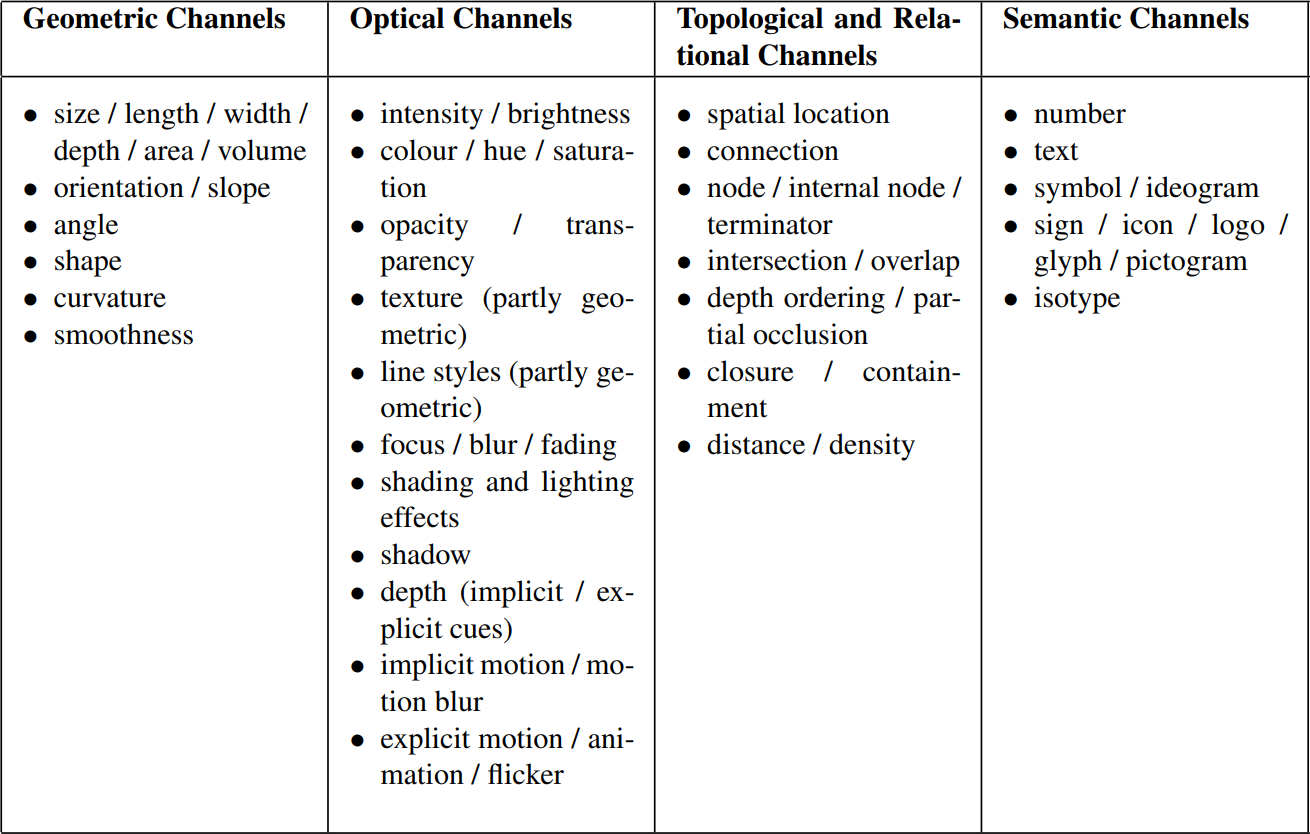
\includegraphics[width=0.7\linewidth]{images/ch7/visualchannels}
\caption{Visual channels presented by Borgo et al.\ \cite{borgo2013glyph}. Refer to Section \ref{sec:reso}} \label{tbl:visualchannels}
\end{table}
\subsubsection*{Resolution Indication} \label{sec:reso}
If area resolution varies across 2D space, it is important to visualize where resolution may lie. We can use visual design variables in order to depict spatial frequency of data. Borgo et al.\ combine multiple visual encoding variables to present a table of visual channels including geometric, optical, topological and relational, and semantic channels \cite{borgo2013glyph}. Refer to Table \ref{tbl:visualchannels}. In Chapter \ref{chap:MultivariateMaps}, we present low resolution indicators by fixing the indicator to outline thickness, size or shadow. In this instance, hidden indicators are mapped to administrative area density. This makes the tool less useful for those already aware of the geospatial structure, however, this could be intrinsic for new users. %Add figure

\begin{figure}[t]
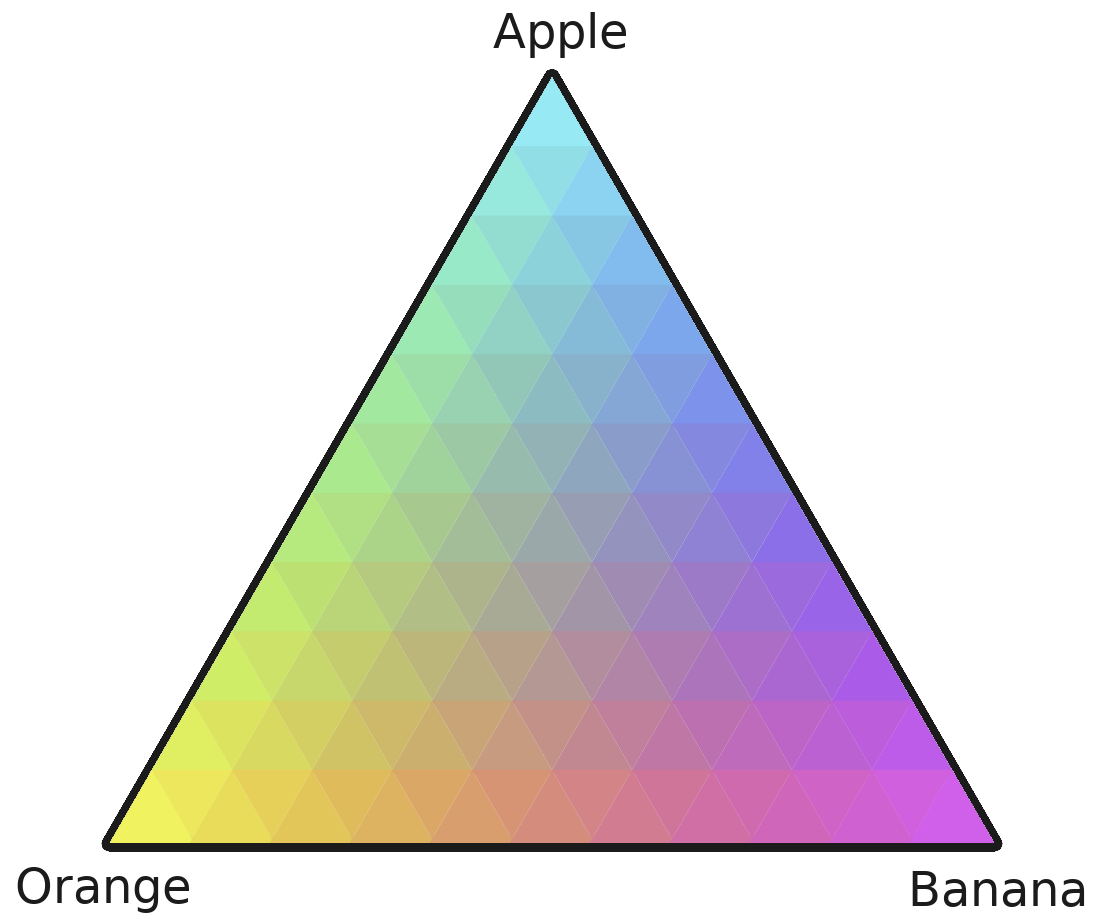
\includegraphics[width=0.4\textwidth]{images/ch7/trivariate}
\caption{A depiction of a trivariate color map. The color map can clearly express the weighting of how values are distributed. By using this with low resolution visualization, we could clearly depict what each area holds at multiple levels of detail. Courtesy of McConchie \cite{mcconchie2018pop}} \label{fig:trivariate}
\end{figure}
\subsubsection*{Uncertainty Visualization}
Uncertainty visualization is a growing aspect of information visualization and applying these techniques to low resolution data is a logical process. Common uncertainty visualization normally uses visual mappings to convey error such as fuzzyness to detract careful analysis. However, when approaching uncertainty in low-resolution visualization, the idea sits in contrast with our attempt to coerce further analysis, causing fuzzyness to be a counter intuitive mapping technique to use. We propose mitigating uncertainty by applying an advanced structure approach to your visual design of choice.
For example, cateorical data could be mapped to present the majority, however a second axis (saturation or opacity for example) can be used to present the percentage of the majority hold.
%If we use color as our visual channel to depict a the most common attribute of `A',`B', and `C', we can apply a bivariate color map to propose a value at the intersection of the highest selection and second highest selection.
We could increase this by modelling a tri-variate color map that depicts the weighting of objects between the three values, presented in Figure \ref{fig:trivariate}. 
There is also work on this technique for higher dimensional data by Cheng et a \cite{cheng2019colormap}.  

\subsection{When to Consider Low Resolution Overviews}
\begin{figure}[t]
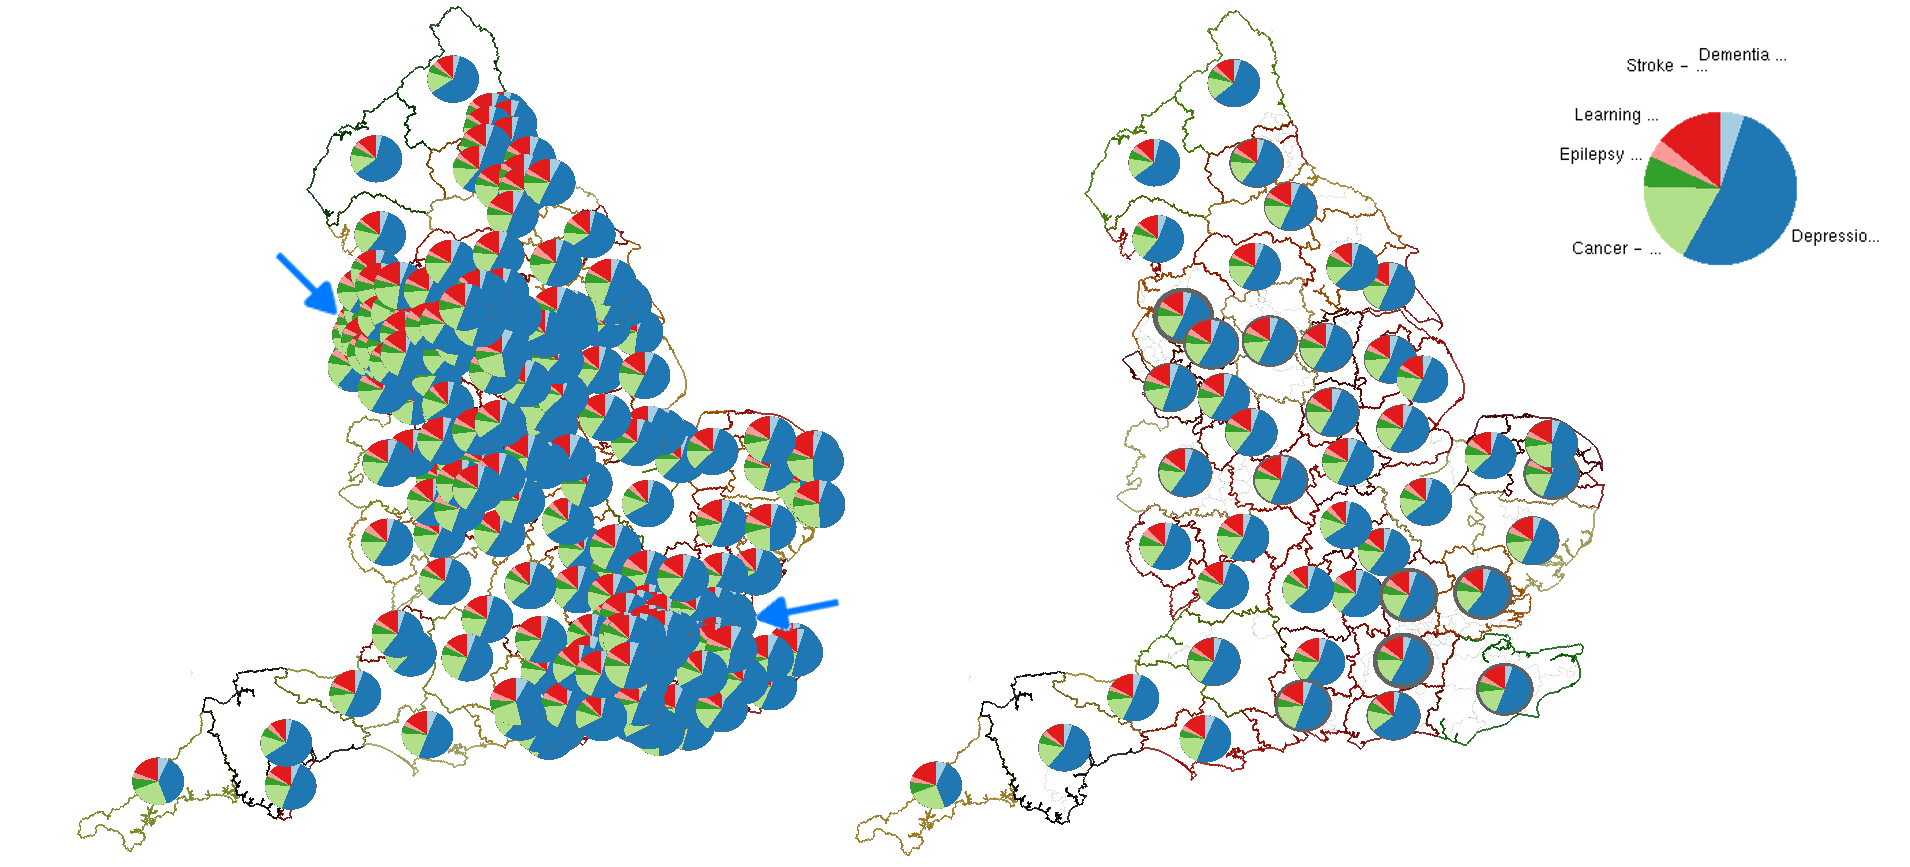
\includegraphics[width=1\textwidth]{images/ch5/ccgsetPie2}
\caption{(left) The representation of population health data based on the Clinical Commisioning Groups (CCGs) of England \cite{publicHealthEngland}. Glyphs that are simply placed at the centroid of each region are over-plotted and occluded around London and Liverpool (indicated by blue arrows). (right) The result using level-of-detail scale-aware maps. Even at a small scale for the figure, we can still clearly differentiate each area's glyph.} \label{fig:occlusion}
\end{figure}

In order to use low resolution overviews, we need to be able to identify when they are appropriate. We use Figure \ref{fig:occlusion} as our first example. \textbf{Occlusion} is likely the easiest criteria to spot. Our example plots glyphs to Clinical Commisioning Groups representing healthcare data. It is possible to reduce occlusion with other methods. For example, Dwyer et al.\ present the Fast Node Overlap Removal (FNOR) algorithm to avoid this \cite{dwyer2005fast}. However, this may not always be useful. In this case, we want to ensure that the glyphs are easily coupled to the geospatial context whilst the FNOR algortihm would remove this entirely in densely populated areas. In this case, areas are amalgamated to make both the glyphs and the underlying values perceivable.

Our second criteria is \textbf{data density}. Even if there is no occlusion, it is still possible for it to become difficult to perceive information. Space-filling techniques such as treemaps can avoid occlusion, but when you have to map millions of events, then the output can result in simple pixel representations of the data. Fekete and Plaisant present a paper working on a treemap for a million items represented \cite{fekete2002interactive}. We can see Figure \ref{fig:ch7treemap} makes it very difficult to see the granular data, which could hide some interesting information. 


\begin{figure}[t]
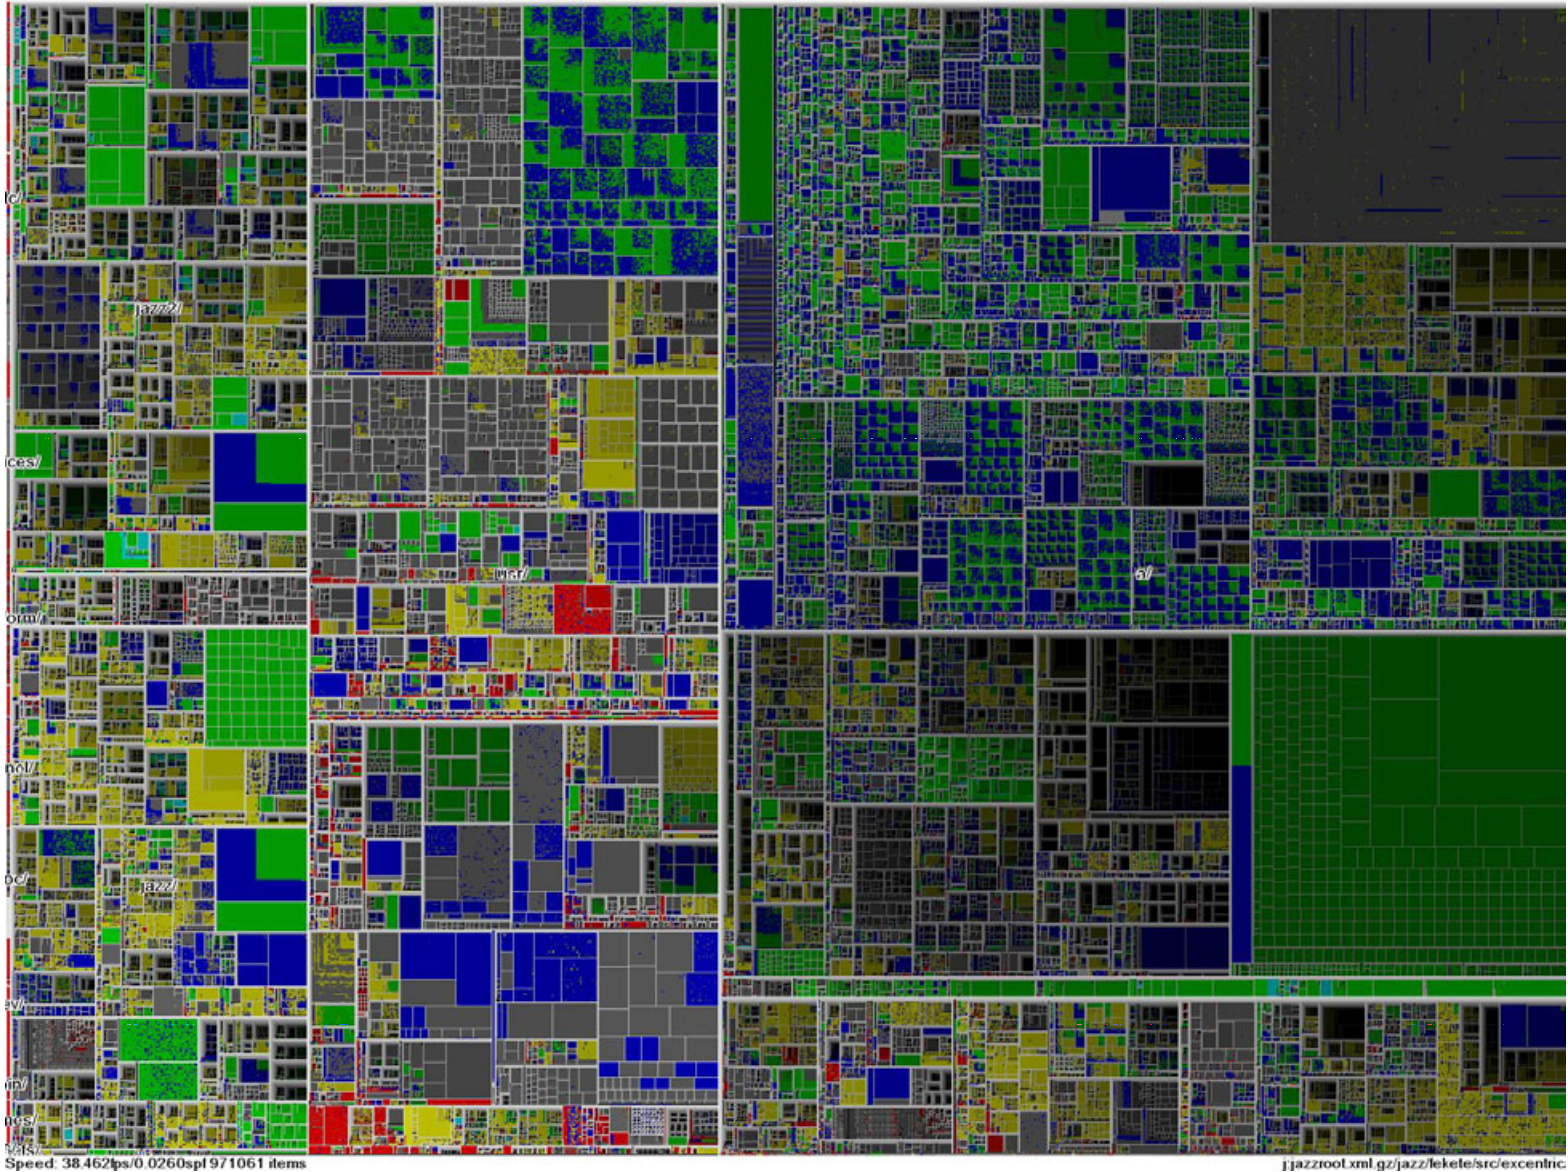
\includegraphics[width=0.7\textwidth]{images/ch7/treemap}
\caption{A treemap depicting a file system of over a million items. Color represents the file type. Image courtesy of Fekete and Plaisant \cite{dwyer2005fast}.} \label{fig:ch7treemap}
\end{figure}
\subsection{Conclusion}
We discuss the concept of reducing data resolution to create low resolution visualization. We look at perception as well as the idea of hiding or anonymising data, and some considerations that need to be taken into account when creating a low resolutions visualization.
\section{Future Work}
During the journey of the thesis, there were many avenues that the thesis could have followed. As such, we dedicate this section to discussing some of these ideas, as well as potential directions a subsequent candidate could follow during their PhD.

With regards to our literature review, We feel we have opened the doors to a range of potential survey papers under the SoS, or meta-survey branch. During the process of the thesis, other related surveys have been published \cite{alharbi2017molecular, alharbi2018sos, rees2019survey}. However, other avenues could be presented such as a Survey of Surveys for Geospatial, Scientific or Computer Graphics.

There are many avenues for future work for the merging algorithm presented in the thesis. Although we use real unit-areas, we would like to test with a broader range of choropleth data. The algorithm still has performance optimizations which could accelerate the speed even further, such as schematization \cite{barkowsky2000schematizing} which could be used to enable better optimization with the drawback of topological continuity being reduced. Other existing formats such as TopoJSON \cite{bostock2018topojson} look at reducing geometry redundancy and could be an excellent subsequent format for the procedure. We worked with 2D coordinate-spaces. A 3D coordinate space would be an exciting direction to take the algorithm and could open new applications for the process. The current termination method revolves around the idea of one area per contiguous region. Updates in the procedure could allow for more user control when it comes to stopping the merge procedure such as for categorical data where the most abstraction is introduced. Alternatively to this, a bi-variate color map could be implemented to display more accurate concordance of underlying values.  The algorithm potentially can apply to any data-sets with geometric boundaries and is open to new data structures. 

There are some limitations to the study we review in Chapter \ref{chap:userStudy}. We found boundary design to be a more significant factor for small area sizes than anticipated. In the pilot study, we found that users had a much better accuracy overall, and comments were made about the area's color changing. This was actually due to the boundary's framing of the pixel, enhancing the perception of color based on the surrounding black contour. We try to control this as carefully as possible, however, this could be examined further in a follow-up study. We use real-world maps and areas. This means we do not control the aspect ratio of the areas, which may lead to more error in some situations such as narrow areas. This is an aspect that can be explored in an alternative study. T1 and T2 could point to a large amount of future research. For example, since we hold data about the location of the presented area and the color seeding, we could look back at what could have influenced the color perception and decision for the area.

For our multivariate implementation in Chapter \ref{chap:MultivariateMaps}. At the moment, we use the raw derived centroid as a placement strategy. Although this removes a lot of density and occlusion, there is still some wasted space. We believe that by adding some overlap removal, we could use space more efficiently, while still avoiding any decoupling problems. Although we present some case studies, the algorithm could be more carefully compared to other glyph placement strategies with a user-study evaluation. We think the use of transitions is a great tool for understanding variation, but it is not always necessary. We feel that there are many avenues for exploring at multiple levels of detail. For example, directly zooming to a glyphs unit area extents may not need to represent zooming, to speed up exploration.

Now that we can improve performance on a second pass-through by saving build instructions to reduce the calculation of neighbor and boundaries, the next step would be to pipe multiple areas to be merged. This would allow the user to constrain area representation to the desired representation further. For example, if we look at the UK, OA's would only merge within their LSOA, and LSOA's would only merge within their MSOA's.

At the Vis 2015 conference, Ribarksy states "When you add dimensions to a problem, all of a sudden it becomes unsolved" \cite{ribarsky2015solved}. Although we extend our technique to take advantage of multivariate data. There are still opportunities to increase the dimensionality by asking for both statistical and temporal data at once.

In order to move full circle (refer to Chapter \ref{chap:SoS}), we must consider scalability as our future work. Although throughout the thesis, we made large leaps in both the scale and performance, we still met some challenges in the area. During our initial testing of the algorithm, we attempted to run the algorithmn on some large datasets, including the output areas of the Wales and England. This dataset held over 180,000 polygons with high complexity vertex lists. Although our algorithm did not fail, the perfomance time became such an issue (days) that we had to terminate before we could see any result. If there was more time, I believe that search for ways to optimize the algorithm in order to make this dataset achievable would be a good next step. Some options for this would be more focus on GPU implementation, multi-threaded processing, and a way to hold contiguous stuctures seperately from the build hierarchy to avoid unecessary recalculation.
